\documentclass{standalone}
\usepackage{PhysicalChemistryNote}
\begin{document}
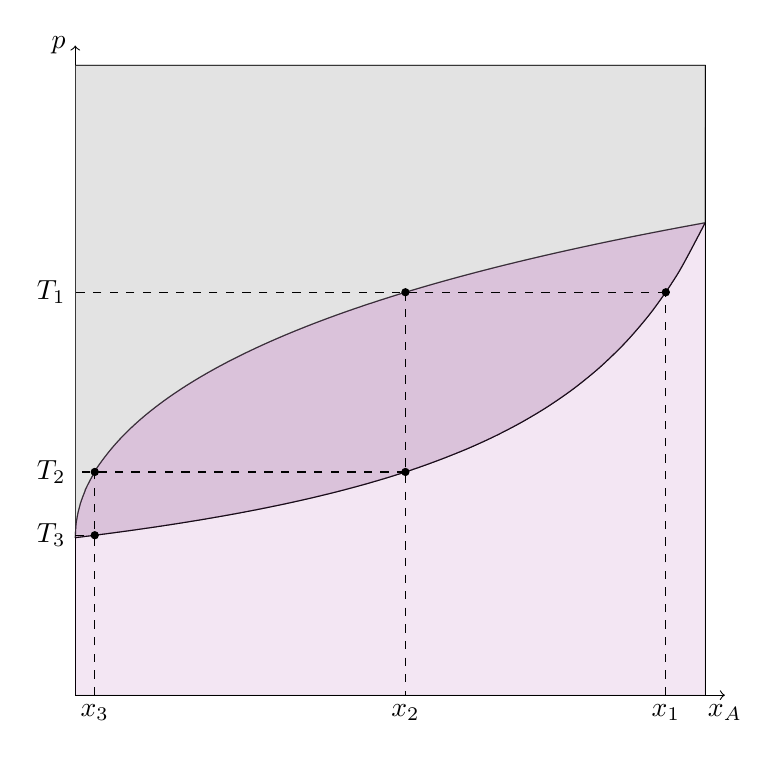
\begin{tikzpicture}
    \draw[->] (0,0) -- (8.25,0) node[below] {$x_A$};
    \draw[->] (0,0) -- (0,8.25) node[left]{$p$};
    \draw[-] (8,0) -- (8,8);
    \draw[-] (0,8) -- (8,8);
    \draw[domain=0:8,samples=1000] plot[smooth](\x,{2*((\x/2)^0.5*(e^(-\x/12)/2+1))/1.2567+2});
    \draw[domain=0:8] plot[smooth](\x,{2/ln(0.25*(4*e+e^(1/3)*(\x/2)-e*(\x/2)))});
    \filldraw[fill=lightgray,opacity=0.25,domain=0:8,samples=1000] plot[smooth](\x,{2*((\x/2)^0.5*(e^(-\x/12)/2+1))/1.2567+2}) -- (8,8) -- (0,8);
    \filldraw[fill=violet,opacity=0.05,domain=0:8,samples=1000] plot[smooth](\x,{2*((\x/2)^0.5*(e^(-\x/12)/2+1))/1.2567+2}) -- (8,0) -- (0,0);
    \filldraw[fill=lightgray,opacity=0.25,domain=0:8] plot[smooth](\x,{2/ln(0.25*(4*e+e^(1/3)*(\x/2)-e*(\x/2)))}) -- (8,8) -- (0,8);
    \filldraw[fill=violet,opacity=0.05,domain=0:8] plot[smooth](\x,{2/ln(0.25*(4*e+e^(1/3)*(\x/2)-e*(\x/2)))}) -- (8,0) -- (0,0);
    \filldraw[fill=violet,opacity=0.15] plot[smooth,domain=0:8](\x,{2/ln(0.25*(4*e+e^(1/3)*(\x/2)-e*(\x/2)))}) -- plot[smooth,domain=8:0,samples=500](\x,{2*((\x/2)^0.5*(e^(-\x/12)/2+1))/1.2567+2});
    \draw[dashed] (7.5,0)--(7.5,5.1167);
    \draw[dashed] (7.5,5.1167)--(0,5.1167);
    \draw[dashed] (4.1928,5.1167)--(4.1928,0);
    \draw[dashed] (4.1928,2.8344)--(0,2.8344);
    \draw[dashed] (0.2477,0)--(0.2477,2.8344);
    \draw[dashed] (0,2.0308)--(0.2477,2.0308);
    \node[below] at (7.5,0) {$x_1$};
    \node[below] at (4.1928,0) {$x_2$};
    \node[below] at (0.2477,0) {$x_3$};
    \node[left] at (0,5.1167) {$T_1$};
    \node[left] at (0,2.8344) {$T_2$};
    \node[left] at (0,2.0308) {$T_3$};
    \fill (7.5,5.1167) circle (1.5pt);
    \fill (4.1928,5.1167) circle (1.5pt);
    \fill (4.1928,2.8344) circle (1.5pt);
    \fill (0.2477,2.8344) circle (1.5pt);
    \fill (0.2477,2.0308) circle (1.5pt);
\end{tikzpicture}
\end{document}